\documentclass[11pt]{article}

\usepackage[margin=1in]{geometry}
\usepackage{booktabs}
\usepackage{graphicx}
\usepackage{hyperref}

\title{FMO Topology Contrast and Lessons: Phase 56.5 Closure Note for HAOS-IIP Biology Telemetry}
\author{Tomislav Rupi\'c \\ Independent Researcher}
\date{April 2026}

\begin{document}

\maketitle

\begin{abstract}
This note closes the initial FMO photosynthesis-telemetry arc in HAOS-IIP as a diagnostic module rather than a forced positive result. Phase 55.2 showed a robust toy-biology PASS on a microtubule-inspired cylindrical lattice: 50/50 runs passed, mean recoverability was $0.916789$, mean protofilament identity was $0.871810$, mean active-null $z$ was $28.705018$, and no controls passed. Phase 56 tested the same spectral-dynamics telemetry family on a compact 7-site FMO-like transfer graph. FMO preserved site identity strongly, but pathway retention and strict control discrimination remained difficult. Sink-aware spectral dynamics improved pathway identity to $0.622057$; explicit pathway-flux restoration raised pathway identity to $0.906155$ but remained a control match; intrinsic directed pathway dynamics improved pass rate to $0.160000$ but lowered pathway identity to $0.671540$. The resulting conclusion is topology sensitivity: HAOS spectral telemetry is strong on structured branch-local lattice scaffolds and diagnostic, but not yet validating, on compact delocalized transfer networks. No molecular FMO, quantum-biology, or photosynthesis claim is made.
\end{abstract}

\begin{figure}[ht]
\centering
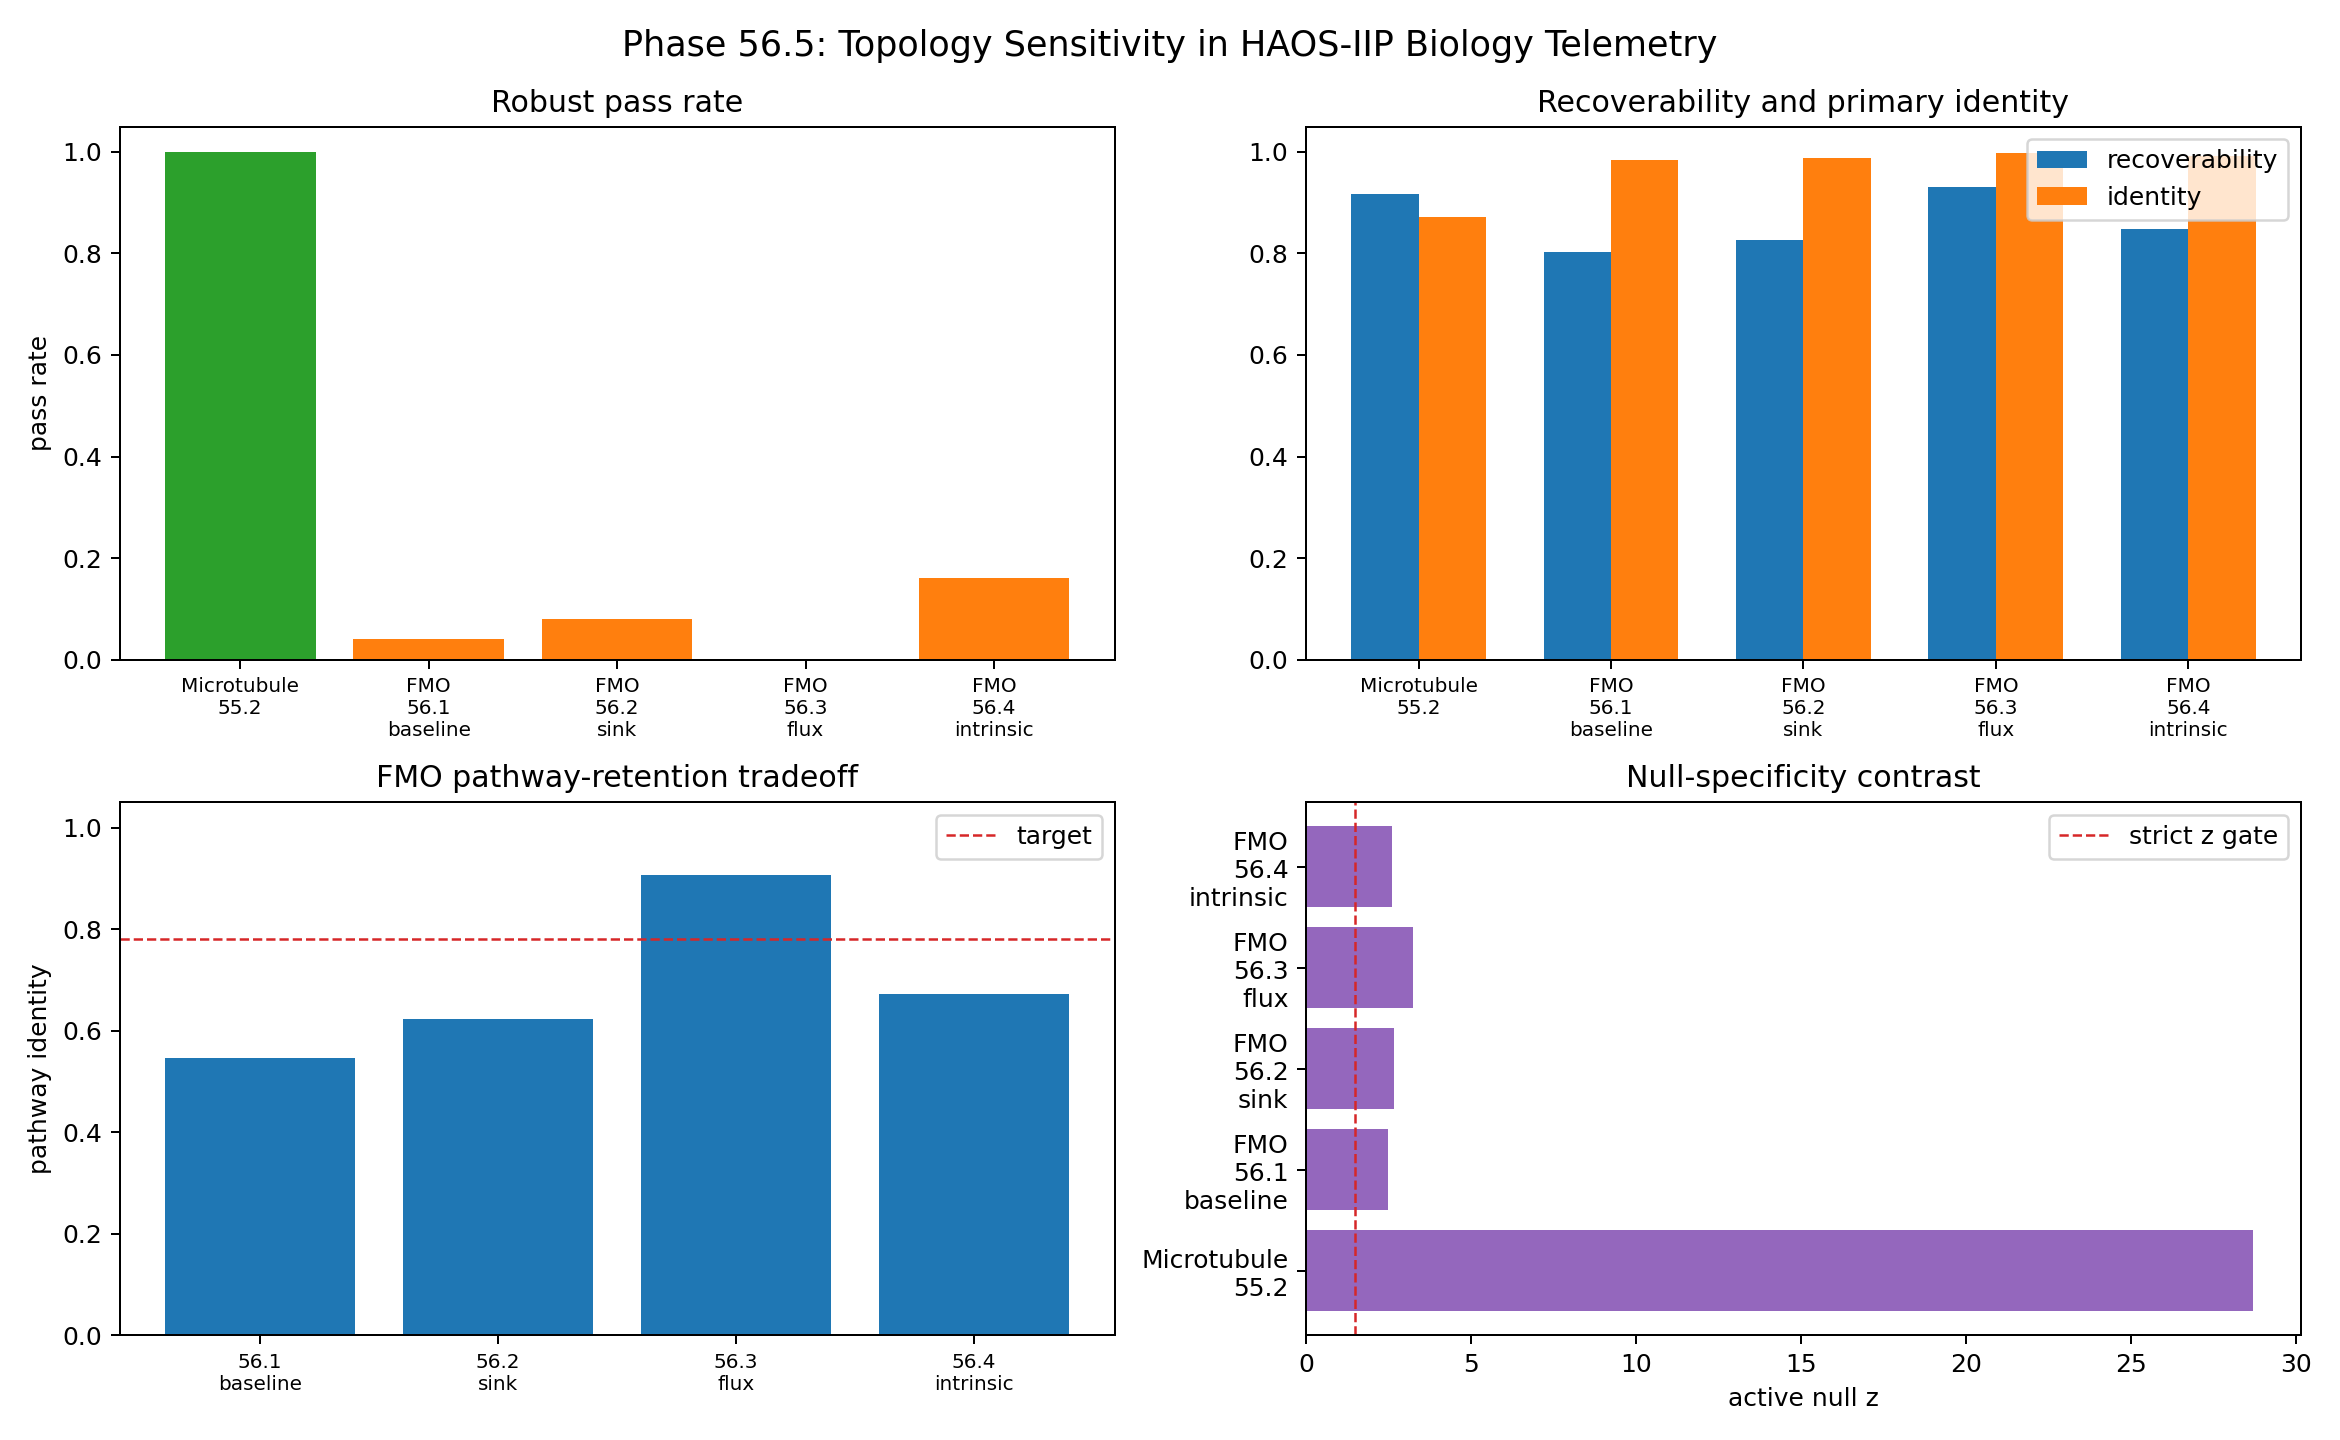
\includegraphics[width=\linewidth]{figures/topology_contrast_56_5.png}
\caption{Phase 56.5 topology contrast. Microtubule 55.2 remains a robust toy PASS, while FMO 56.1--56.4 maps a tradeoff between site identity, pathway retention, and strict control specificity.}
\end{figure}

\section{Scope}

This is a closure note for the initial FMO telemetry sidecar:
\begin{quote}
\texttt{experiments/biology/fmo\_photosynthesis\_telemetry/}
\end{quote}

It compares that sidecar against the Phase 55.2 microtubule robustness result:
\begin{quote}
\texttt{experiments/biology/microtubule\_lattice\_demo/}
\end{quote}

The scope is intentionally narrow. The FMO graph is a toy weighted transfer network based on a standard 7-site FMO-like coupling pattern. It is not a molecular simulation, exciton-transport model, quantum-biology result, or photosynthesis claim.

\section{Comparison}

\begin{center}
\begin{tabular}{lrrrrrl}
\toprule
System & Runs & Pass rate & Recoverability & Identity & Pathway & Status \\
\midrule
Microtubule 55.2 & 50 & 1.000000 & 0.916789 & 0.871810 & n/a & robust PASS \\
FMO 56.1 baseline & 50 & 0.040000 & 0.803724 & 0.984934 & 0.546597 & diagnostic fail \\
FMO 56.2 sink & 50 & 0.080000 & 0.827528 & 0.988291 & 0.622057 & diagnostic fail \\
FMO 56.3 flux & 50 & 0.000000 & 0.930908 & 0.998190 & 0.906155 & control match \\
FMO 56.4 intrinsic & 50 & 0.160000 & 0.848259 & 0.991098 & 0.671540 & productive falsifier \\
\bottomrule
\end{tabular}
\end{center}

\section{Topology Sensitivity}

The microtubule lattice and the FMO-like transfer graph behave differently under the same telemetry discipline.

The microtubule sidecar has repeated cylindrical structure, protofilament-level identity, and multi-scale local couplings. Under the level-5 null ladder, its observed dynamics remain recoverable and identity-preserving while strict controls do not pass.

The FMO sidecar is compact and delocalized. It preserves site identity easily, but pathway identity and branch-specific control discrimination are harder. This is not a failure of the audit machinery. It is the machinery exposing where a substrate is too small, too globally coupled, or too easily matched by controls.

\section{FMO Lessons}

Phase 56.1 established the baseline falsifier. Site identity was strong, but pathway retention was weak and controls remained competitive.

Phase 56.2 added sink-aware and hybrid address variants. The best variant, sink-aware spectral dynamics, improved pathway identity from $0.546597$ to $0.622057$, but pass rate stayed low.

Phase 56.3 added explicit signed-flux restoration along the declared pathway edges. This solved the pathway-retention metric, reaching $0.906155$, but it also made the engineered pathway term easy for controls to exploit. This produced a control-match result, not a validation result.

Phase 56.4 replaced strong explicit flux restoration with weaker intrinsic directed and temporal pathway dynamics plus a level-6 directed trajectory null. This improved pass rate to $0.160000$ but reduced pathway identity to $0.671540$.

The tradeoff is informative:
\begin{quote}
strong explicit pathway terms preserve the declared pathway but leak to controls; weaker intrinsic pathway terms reduce over-engineering but lose pathway fidelity.
\end{quote}

\section{Closure Decision}

The correct decision is to stop tuning FMO for a green result. The initial FMO arc should be frozen as a productive falsifier.

Current interpretation:
\begin{itemize}
\item HAOS spectral telemetry is robust on the microtubule toy lattice.
\item HAOS spectral telemetry is diagnostic but not yet validating on the compact FMO-like transfer graph.
\item The FMO bottleneck is branch-specific pathway discrimination, not simple recoverability or site identity.
\item Future FMO work should require a new transfer-state model or a sharper branch-specific control-discrimination metric.
\end{itemize}

\section{Non-Claims}

This release does not claim:
\begin{itemize}
\item molecular FMO dynamics;
\item exciton transport recovery;
\item quantum-biology or photosynthesis validation;
\item universal biological telemetry closure;
\item that FMO should be made to pass by parameter tuning.
\end{itemize}

The value of Phase 56 is the contrast: robust microtubule specificity versus FMO pathway/control tension.

\section{Artifacts}

Primary artifacts:
\begin{itemize}
\item \texttt{experiments/biology/fmo\_photosynthesis\_telemetry/fmo\_topology\_contrast\_56\_5.md}
\item \texttt{experiments/biology/fmo\_photosynthesis\_telemetry/run\_topology\_contrast\_summary.py}
\item \texttt{experiments/biology/fmo\_photosynthesis\_telemetry/figures/topology\_contrast\_56\_5.png}
\item \texttt{experiments/biology/microtubule\_lattice\_demo/microtubule\_spectral\_robustness\_55\_2.md}
\end{itemize}

\end{document}
